\chapter{Automatic Text Summarization}
\thispagestyle{fancy}
\label{chap:Automatic Text Summarization}

\noindent
Unter Kenntnis der theoretischen Grundlagen werden die Ausführungen zur \ac{ATS} in diesem Kapitel ausgeweitet, basierend auf den einordnenden Worten aus der Einleitung. Dabei werden die grundlegenden Informationen vollständigerweise zusammengefasst und mithilfe des neu gewonnenen Wissens nochmalig eingeordnet. Darüber hinaus wird insbesondere der Forschungsstand vertieft, vergleichbare Arbeiten analysiert und daraufhin selbst eine Architektur konzipiert.\\


\section{Typisierung von Systemen}
\noindent
Es ist bereits bekannt, dass die \ac{ATS} verschiedenartig typisiert werden kann. Dies wird in der nachstehenden Liste ersichtlich. Dabei wird die Typisierung der in dieser Arbeit behandelten \ac{ATS} entsprechend der Zielsetzung markiert. Faktoren, welche die entsprechenden Entscheidungen herbeiführen, werden anschließend hinreichend erläutert \cite[S.~5]{GAM16}.

\begin{itemize}
	\item Extractive vs. \textbf{\textcolor{purple}{Abstractive}}
	\item \textbf{\textcolor{purple}{Generic}} vs. Query-Focused
	\item \textbf{\textcolor{purple}{Single-Document}} vs. Multi-Document
	\item \textbf{\textcolor{purple}{Supervised}} vs. Unsupervised
	\item Mono-/ \textbf{\textcolor{purple}{Multi-}}/ Cross-\textbf{\textcolor{purple}{Lingual}}
\end{itemize}

\noindent
Zunächst muss zwischen einer extraktiven und einer abstraktiven Methodik differenziert werden. Dabei ist zugleich zu definieren, ob Zusammenfassungen eher allgemein oder abfragebasiert generiert werden sollen. Dies wird von den individuellen Anforderungen an die einzusetzende \ac{ATS} bedingt und bestimmt. Von weiteren Erklärungen zu den genannten Methodiken wird an dieser Stelle abgesehen, weil die entsprechenden Grundlagen entweder bereits erklärt wurden oder im weiteren Verlauf der Arbeit nicht mehr relevant sein werden.
\newpage

\noindent
Bevor ein \ac{ATS}-System tatsächlich entwickelt werden kann, sind weitere Eigenarten zu identifizieren. Dies betrifft fortan insbesondere die Beschaffenheit der verfügbaren Daten, welche als Entscheidungsfaktor in die Typisierung der \ac{ATS} eingehen. Daher ist zu ergründen, ob Zusammenfassungen auf nur einem oder mehreren Dokumenten basieren. Zudem ist anhand der verfügbaren Daten abzulesen, ob das Training überwacht oder unüberwacht stattfinden kann. Zuletzt ist ein \ac{ATS}-System durch die Sprache(n) der zugeführten Daten limitiert \cite[S.~5]{GAM16}.\\

\noindent
Technisch sei zusammengefasst, dass bei der \ac{ATS} eine Eingabesequenz $x = [x_{1}, ..., x_{n}]$ in eine Ausgabesequenz $y = [y_{1}, ..., y_{m}]$ überführt wird, wobei $n$ die Eingabelänge und $m$ die Ausgabelänge ist. Dabei gilt stets $m$ \textless \, $n$ mit dem Ziel $P(y \mid x)$. Die wesentlichen Herausforderungen bestehen dabei aus dem \ac{NLU} und der \ac{NLG} \cite[S.~32-33]{NIT19}.


\section{Vertiefung des Forschungsstands}
\noindent
Nun wird der einleitend bereits umrissene Forschungsstand für den soeben eingegrenzten \ac{ATS}-Typ vertieft. Neben vielversprechenden Ansätzen der letzten Jahre, welche mitunter auf \ac{RNN}, \ac{LSTM} und \ac{RL} basierten, etablierten sich im \ac{SOTA} seit 2018 bekanntermaßen Transformer. Nachfolgend wird daher beschrieben, wie Transformer bislang im Kontext der \ac{ATS} eingesetzt wurden und wie Verbesserungen erzielt werden können. Hierfür werden die eingangs aufgelisteten vergleichbaren Arbeiten nun mit dem neu gewonnenen Wissen ausführlicher thematisiert und eingeordnet.\\

\noindent
Yang et al. übertrafen 2019 den \ac{SOTA} im Bereich der abstraktiven \ac{ATS} mithilfe einer Encoder-Decoder-Architektur, wobei der Encoder durch einen vortrainierten \ac{BERT} und der Decoder durch einen zufällig initialisierten Transformer repräsentiert wurde. Eine wesentliche Erkenntnis hierbei war die Multifunktionsfähigkeit von \ac{BERT} zur \ac{NLU} und zur \ac{NLG} \cite{YAN19}.\\

\noindent
Nitsche befasste sich 2019 ebenfalls mit abstraktiver \ac{ATS}. Dabei verwendete er in seiner Architektur ebenfalls \ac{BERT}, jedoch in einer multilingual vortrainierten Version. Damit gelang ihm der Versuch, die Architektur trotz mangelnder Ressourcen im deutschsprachigen \ac{NLP}-Bereich auf die deutsche Sprache zu adaptieren. Aufgrund nicht verfügbarer Daten lässt sich keine weitergehende Aussage über die Qualität seiner Ergebnisse treffen \cite{NIT19}.
\newpage

\noindent
Rothe et al. verfolgten 2020 eine Transformer-to-Transformer-Architektur zur \ac{ATS}. Dabei werden die entsprechenden Encoder und Decoder in jedem Experiment durch vortrainierte Transformer repräsentiert, darunter beispielsweise \ac{BERT}-to-\ac{BERT}, \ac{XLM-R}-to-\ac{XLM-R} oder sogar \ac{BERT}-to-\ac{XLM-R}. Hierbei kamen Rothe et al. zu der Erkenntnis, dass monolinguales Fine-Tuning zu besseren Resultaten führt. Zugleich wird deutlich, dass multilinguales Vortraining profitabel sein kann. Die folgenden \ac{ROUGE}-Scores können als \ac{SOTA} registriert werden: R-Recall: 15.96, R-Precision: 10.34, R-Measure: 12.22 \cite{ROT20}.\\

\noindent
In den soeben vertieften Publikationen wird ersichtlich, dass gemäß \ac{TL} vortrainierte Transformer sowohl als Encoder als auch als Decoder genutzt werden können, stets unter gegebener Austauschbarkeit. Die sprachtechnische Adaption hingegen wurde bislang nur unzulänglich oder nicht-öffentlich erprobt. Daher wird in dieser Arbeit eine Architektur zur \ac{ATS} eingeführt, welche die Fortschritte aufgreift sowie vorhandene Unzulänglichkeiten verbessert. Hierfür werden Transformer-Kombinationen mit besonderem Fokus auf die deutschsprachige Adaption erprobt. Gemäß dem \ac{SOTA} werden \ac{BERT}, \ac{XLM-R} und \ac{BART} ausgewählt, nicht hingegen \ac{ELMo} und \ac{GPT}.


\section{Konzeption einer Architektur}
\noindent
Mit dem bisherigen Wissen wird nun eine Architektur konzipiert. Diese ist als \ac{TF2TF} zu verstehen. Dabei wird sowohl der Encoder als auch der Decoder durch eine eigenständige gemäß \ac{TL} vortrainierte \ac{DLR} repräsentiert. Aufgrund der bereits beschriebenen Grundlagen wird nun die weitergehende Konfiguration der Architektur definiert. Hierbei gibt es unter anderem die folgenden beiden Möglichkeiten, um den Encoder zum \ac{NLU} und den Decoder zur \ac{NLG} zu initialisieren \cite[S.~2]{ROT20}.\\

\noindent
Einerseits ist es möglich, den Encoder und den Decoder jeweils mit einer autarken \ac{DLR} zu initialisieren, beispielsweise den Encoder mit \ac{BERT} und den Decoder mit \ac{GPT}. Andererseits ist es aber auch möglich, sowohl den Encoder als auch den Decoder mit dem gleichen Checkpoint einer \ac{DLR} zu initialisieren, welche ursprünglich nur als Encoder trainiert wurde, beispielsweise mit \ac{BERT}. Gemäß \ac{TL} wird so im Kontext von \ac{NLP} und \ac{ATS} das Neuerlernen einer Sprache umgangen. Aufgrund der Verfügbarkeit von \ac{BERT} wird in der Folge nur letztere Möglichkeit betrachtet. Die folgenden Ausführungen sind in \autoref{pic:EncoderDecoderBert} visualisiert \cite[S.~2-3]{ROT20}.\\

\begin{figure}[h!]
  \centering
  \fbox{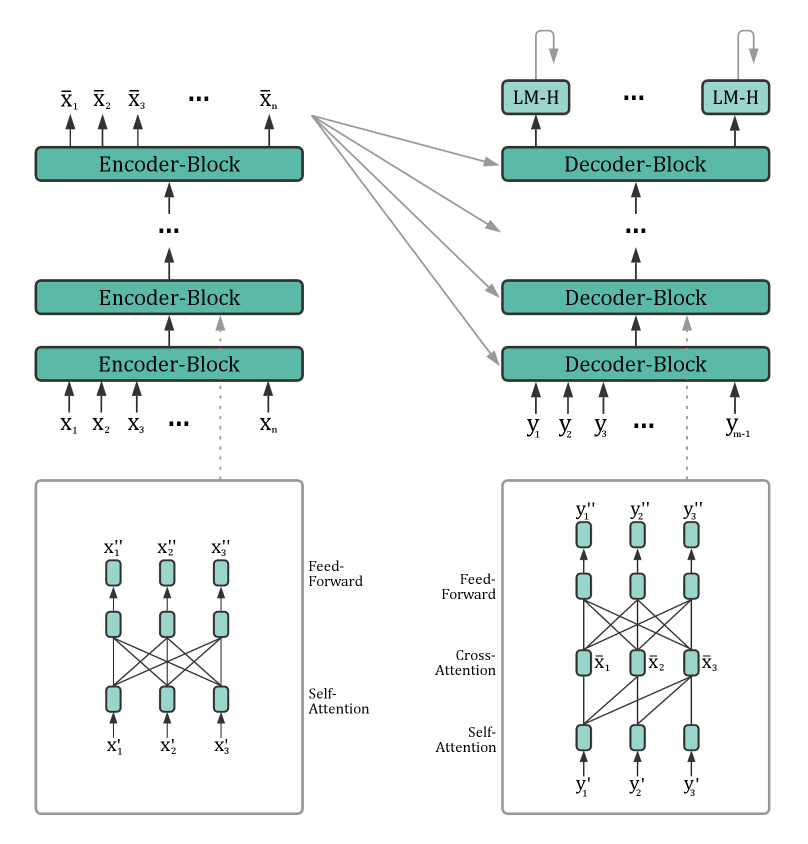
\includegraphics[width=0.8\linewidth]{./source/images/encoderdecoderbert.png}}
  \caption{Sequence-to-Sequence-Transformer-Modell mit BERT \cite{VON20}.}
  \label{pic:EncoderDecoderBert}
\end{figure}

\noindent
Die Gewichte der bidirektionalen Self-Attention-Schichten und der Feed-Forward-Schichten aller Encoder-Blöcke werden mit den vortrainierten Gewichten von \ac{BERT} initialisiert. Dabei kann der Encoder schlichtweg als \ac{BERT} in seiner Reinform verstanden werden. Der Decoder hingegen bedarf mindestens der nachstehenden Anpassungen \cite{VON20}.\\

\noindent
Zunächst werden sogenannte Cross-Attention-Schichten zwischen den Self-Attention-Schichten und den Feed-Forward-Schichten aller \ac{BERT}-Blöcke eingeführt, um die kontextbasierten Sequenzen verarbeiten zu können. Die Gewichte der Cross-Attention-Schichten werden hierbei zufällig initialisiert \cite{VON20}.
\newpage

\noindent
Zudem werden die bidirektionalen Self-Attention-Schichten zu unidirektionalen Self-Attention-Schichten transformiert, um der autoregressiven Funktionsweise eines Decoders gerecht zu werden. Bei der autoregressiven \ac{NLG} wird angenommen, dass die Wahrscheinlichkeitsverteilung einer Sequenz in das Produkt der bedingten nächsten Wortverteilungen zerlegt werden kann \cite{VON20}. Beide Attention-Schichten basieren auf den gleichen Projektionen aus Key, Query und Value, weshalb die Gewichte dieser Schichten weiterhin mit den Werten von \ac{BERT} initialisiert werden können. Die unidirektionalen Self-Attention-Schichten berücksichtigen nun nur noch vorangegangene Token, nicht mehr auch die nachstehenden Token. Dies führt zu veränderten Ausgabevektoren im Vergleich zum ursprünglichen \ac{BERT}, obwohl sie die gleichen Gewichte teilen \cite[S.~2]{ROT20}.\\

\noindent
Zuletzt wird dem Decoder eine sogenannte Language-Model-Head-Schicht hinzugefügt, dessen Gewichte mit denen des gewählten Word Embeddings initialisiert werden. Hierbei handelt es sich erneut um \ac{BERT}. Es wird deutlich, dass sich der Encoder und der Decoder viele Gewichte teilen können. Dies führt zu einer erheblichen Reduktion des Speicherbedarfs, während die Qualität anschließender \ac{NLP}-Aufgaben nahezu unverändert bleibt \cite[S.~2]{ROT20}.\\

\noindent
Die Textinhalte der Datengrundlage bedürfen überdies keiner weitergehenden Vorverarbeitung im herkömmlichen Sinne. Diese ist bekanntermaßen sehr individuell und stark modellabhängig. Unter Verwendung der als sehr robust geltenden Transformer-Architekturen entfällt daher die sonst übliche Textbereinigung sowie die Textnormalisierung. Dies unterliegt der Annahme, dass Transformer-Architekturen potenziell aus jeder Eigenart ein relevantes Feature schaffen können, welches das spätere Ergebnis begünstigt. Von der zugeführten Interpunktion und den vielfältigen Wortformen wird sich indes erhofft, potenzielle Mehr- oder Uneindeutigkeiten zu minimieren. Das Fine-Tuning sollte darüber hinaus stets unter gleichen Bedingungen wie das initiale Training stattfinden. Gleichzeitig sinkt hierdurch der vorverarbeitende Aufwand und damit auch etwaige Wartezeiten bei der praktischen Anwendung bereits trainierter Modelle in Echtzeit. Dennoch ist es möglich, bestimmte Vorverarbeitungsschritte a posteriori zu implementieren. Die Auswirkungen auf das Modell und die entsprechenden Ergebnisse würden somit zugleich messbar.
\newpage

\noindent
In der sonstigen technischen Vorbereitung ist weiterhin ein Tokenizer zu definieren. Dieser entstammt ebenfalls \ac{BERT} und berücksichtigt Groß- und Kleinschreibung. \ac{BERT} kann Sequenzen bis zu einer maximalen Länge von 512 Token verarbeiten. Dies unterschreitet zwar die durchschnittliche Textlänge der beschriebenen Korpora, kann jedoch unter der Annahme, dass wichtige Informationen zumeist am Anfang von Texten stehen, akzeptiert werden \cite{VON20}.\\

\noindent
Von einer schlichten Erhöhung der maximalen Tokenlänge ist indes abzuraten, da hierbei ein quadratischer Anstieg der Rechenzeit und des Speicherbedarfs zu erwarten ist. Zudem wurde \ac{BERT} ausschließlich auf Texten mit einer maximalen Tokenlänge von 512 trainiert. Ein denkbarer Lösungsansatz, welcher an dieser Stelle nur genannt sei, ist der sogenannte Sliding-Window-Approach. Hierbei besteht jedoch die Gefahr, dass langfristige Abhängigkeiten verloren gehen. Zuvor sind außerdem entsprechende Testläufe durchzuführen. Weiterhin existieren Ansätze wie etwa Longformer oder auch Big Bird, welche die Verarbeitung langer Sequenzen verfolgen \cite{ZAH21}. Diese versuchen zugleich, lineare Komplexität zu erreichen, beispielsweise mithilfe lokaler Attention-Mechanismen, die wiederum mit globaler Attention verknüpft sind \cite{BEL20}. Ein eher anwendungsbezogener Workaround besteht hingegen darin, den jeweils eingehenden Rohtext alle 512 Token zu unterteilen, die Subtexte einzeln zusammenzufassen und die Zusammenfassungen zu konkatenieren. Dies betrifft jedoch nicht das eigentliche Training \cite[S.~2]{DIN20}.\\

\noindent
Texte werden also zusammenfassend in den nachfolgenden Schritten jeweils nach 512 Token abgeschnitten. Die maximale Tokenlänge der entstehenden Zusammenfassungen wird auf 128 limitiert. Anpassungen, welche etwa im Laufe der experimentgetriebenen Entwicklung und Optimierung an Potenzial gewinnen, werden an den entsprechenden Stellen ergründet und evaluiert.

\section{Adaption der Sprache}
\noindent
TODO
